\section{Processo implementativo}
\label{sec:chapter_3_section_5}

Con processo implementativo di un \emph{Plugin} si intende la formalizzazione delle fasi progettuali.
La formalizzazione del procedimento traccia metodologicamente una sequenza di passi da seguire:
(a) studio della geometria, (b) definizione della funzione di render 2D, (c) definizione della funzione di render 3D,
 (d) instanziazzione nel catalogo, (e) testing nella scena.


\subsection{Studio della geometria}
Nella prima fase implementativa dopo aver scelto quale oggetto andare a modellare all'interno del framework,
si passa ad uno studio della geometria dell'oggetto reale (Figura \ref{fig:confronto} - a).
In presenza di un modello complesso bisogna pensare a come realizzarlo cercando di scinderlo in parti geometriche semplici.
Ad esempio analizzando l'oggetto estintore, esso è composto da una geometria complessa che è scindibile in parti geometriche
semplici, come un cilindro più una semisfera per il corpo centrale (Figura \ref{fig:confronto} - b). Si segue questa procedura
per tutte le componenti fino alla realizzazione dell'intero modello virtuale (Figura \ref{fig:confronto} - c).\\

   \begin{figure}[htbp]
   \begin{center}
   \begin{tabular}{ccc @{\hspace{2cm}} ccc}
   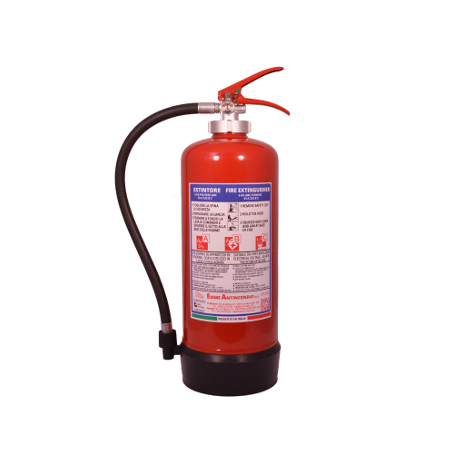
\includegraphics[width=3.8cm]{images/estintore2} &
   
\includegraphics[width=3.8cm]{images/esplosoestintore} &
   
\includegraphics[width=3.8cm]{images/estintore}\\
    (a) & (b) & (c)\\
   \end{tabular}
   \end{center}
   \caption{(a) Foto modello reale, (b) Modello 3D esploso in elementi geometri semplici, (c) Modello 3D virtuale}
   \label{fig:confronto}
   \end{figure}

Dopo aver scomposto l'oggetto in elementi geometrici semplici, è necessario reperire le informazioni come
larghezza, profondità, altezza e altri dati utili alla modellazione.


\subsection{Definizione funzione di render 2D}
La funzione di render 2D, attraverso il linguaggio \emph{SVG} (Scalable Vector Graphics),
consente di visualizzare oggetti di grafica vettoriale e, pertanto, di gestire immagini scalabili dimensionalmente.
Questa definizione consente di inserire all'interno del Virtual DOM della content-area la rappresentazione 2D dell'oggetto
aggiornando l'area interessata del canvas.
In questo modo il Plugin viene visualizzato all'interno di Metior durante la visualizzazione in 2D della scena.\\


\lstset{
    basicstyle=\fontfamily{cr}\selectfont\footnotesize\color{black},
    numbers=none, % where to put the line-numbers
    numberstyle=\tiny, % the size of the fonts that are used for the line-numbers
    backgroundcolor=\color{white},
    showspaces=false, % show spaces adding particular underscores
    showstringspaces=false, % underline spaces within strings
    showtabs=false, % show tabs within strings adding particular underscores
    frame=single, % adds a frame around the code
    tabsize=2, % sets default tabsize to 2 spaces
    captionpos=b, % sets the caption-position to bottom
    breaklines=true, % sets automatic line breaking
    breakatwhitespace=false,
    xleftmargin=17pt,
    framexleftmargin=17pt,
    framexrightmargin=17pt,
    framexbottommargin=5pt,
    framextopmargin=5pt
}
\begin{lstlisting}[
                   numbers=left,
                   frame=trBL,
                   basicstyle=\tiny,
                   caption={Definizione della funzione di render 2D},
                   label=struttura]
render2D: function (element, layer, scene) {
 return (
  <g transform={'translate(${-RADIUS/(RADIUS/2)},
                           ${-(RADIUS+5)/(RADIUS/2)})'}>
   <ellipse key="1" cx="0" cy="0" rx={RADIUS+5} ry={RADIUS}
   style={{stroke: element.selected ? '#0096fd' : '#000',
           strokeWidth: "2px", fill: "#ff0000"}}/>
   <line key="2" x1={0} x2={0} y1={RADIUS} y2={2*RADIUS}/>
   <line key="3" x1={-RADIUS/2+.15*RADIUS} x2={-RADIUS/2+RADIUS/2}
                 y1={1.2*RADIUS} y2={2* RADIUS}/>
   <line key="4" x1={0} x2={-RADIUS/2+.85*RADIUS}
                 y1={2*RADIUS} y2={1.2*RADIUS}/>
   <text key="5" cx={RADIUS} cy={RADIUS}
    transform={ 'translate(${RADIUS/8}, ${0})
                 scale(1,-1) rotate(${angle/2})'}>
     {element.type}
   </text>
  </g>
 )
},
\end{lstlisting}
\newpage

\subsection{Definizione funzione di render 3D}
La funzione di render 3D definisce attraverso una porzione di codice scritto in Javascript ed utilizzando
la libreria open-source \emph{Threejs}, un modello 3D del Plugin;
questa definizione ne consente pertanto la rappresentazione all'interno di Metior durante la visualizzazione in 3D della scena.\\


\begin{lstlisting}[
                   numbers=left,
                   frame=trBL,
                   basicstyle=\tiny,
                   caption={Definizione della funzione render 3D},
                   label=struttura]
 render3D: function (element, layer, scene) {

  var red = new Three.MeshLambertMaterial({color: 0xff0000});

  var fireExtinguisher = new Three.Object3D();

  var bodyGeometry = new Three.CylinderGeometry(0.1, 0.1, 0.5, 32);
  var body = new Three.Mesh(bodyGeometry, red);
  body.position.set(0, 1, 0);
  fireExtinguisher.add(body);

  var geometrySphereUp = new Three.SphereGeometry(0.1, 32, 32);
  var sphereUp = new Three.Mesh(geometrySphereUp, red);
  sphereUp.position.set(0, 0.25, 0);
  body.add(sphereUp);

  ...

  let value = new Three.Box3().setFromObject(fireExtinguisher);

   let deltaX = Math.abs(value.max.x - value.min.x);
   let deltaY = Math.abs(value.max.y - value.min.y);
   let deltaZ = Math.abs(value.max.z - value.min.z);

   if (element.selected) {
     let bbox = new Three.BoxHelper(fireExtinguisher, 0x99c3fb);
     bbox.material.linewidth = 5;
     bbox.renderOrder = 1000;
     bbox.material.depthTest = false;
     fireExtinguisher.add(bbox);
   }

   fireExtinguisher.rotation.y += -Math.PI / 2;
   fireExtinguisher.position.y += -HEIGHT / 1.15 + newAltitude;
   fireExtinguisher.position.z += 10;

   fireExtinguisher.scale.set(RADIUS/deltaX,RADIUS/deltaX,HEIGHT/deltaY);

   return Promise.resolve(fireExtinguisher);
 }
\end{lstlisting}
\newpage

\subsection{Instanziazione nel catalogo}
Dopo aver implementato un Plugin è necessario, al fine di poterlo inserire all'interno di una scena, instanziarlo
all'interno del \emph{Plugin Catalog}.\\
\begin{lstlisting}[
                   numbers=left,
                   frame=trBL,
                   basicstyle=\tiny,
                   caption={Instanziazione del Plugin nel Catalogo},
                   label=struttura]
import {Catalog} from 'react-planner';
...
import estintore from './items/estintore/estintore';
...
catalog.registerElement(estintore);
...
export default catalog;
\end{lstlisting}

\subsection{Testing nella scena}
La fine del processo richiede il testing del nuovo \emph{Plugin} implementato, testandolo all'interno
di una scena per verificare che le caratteristiche, geometriche e dimensionali corrispondando con quelle
del modello reale dal quale si è preso spunto per la realizzazione del modello virtuale.\\
